% !TEX TS-program = xelatex
% !TEX encoding = UTF-8 Unicode
\documentclass[aspectratio=169,11pt]{beamer}

\usetheme{Madrid}
\usecolortheme{default}
\setbeamertemplate{navigation symbols}{}
\setbeamertemplate{caption}[numbered]

\usepackage{fontspec}
\setsansfont{Latin Modern Sans}
\setmainfont{Latin Modern Roman}
\setmonofont{Latin Modern Mono}
\usepackage{graphicx}
\usepackage{booktabs}
\usepackage{array}

\definecolor{accentblue}{RGB}{22,58,105}
\definecolor{accentteal}{RGB}{20,122,112}
\definecolor{accentorange}{RGB}{232,116,28}
\definecolor{softblue}{RGB}{238,246,255}
\definecolor{ink}{RGB}{25,33,45}

\setbeamercolor{title}{fg=white}
\setbeamercolor{subtitle}{fg=white}
\setbeamercolor{frametitle}{fg=white,bg=accentblue}
\setbeamercolor{structure}{fg=accentblue}
\setbeamercolor{block title}{fg=white,bg=accentblue}
\setbeamercolor{block body}{fg=ink,bg=softblue}

\newcommand{\archfig}[1][0.68\textheight]{%
  \makebox[\textwidth][c]{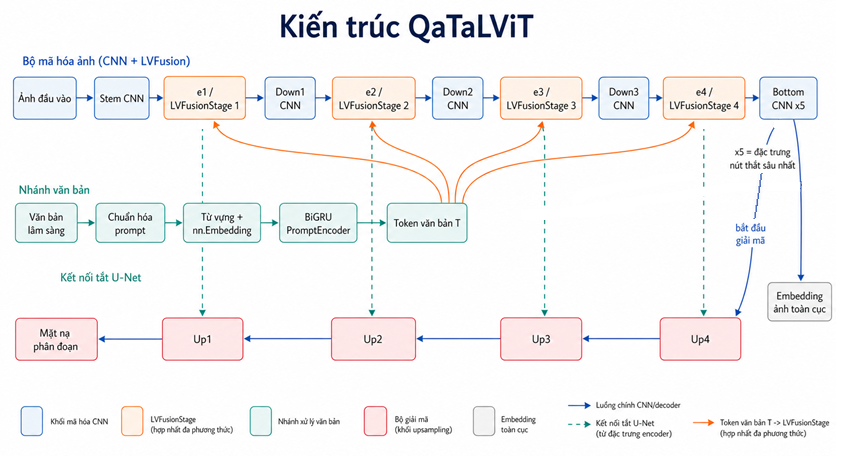
\includegraphics[width=0.96\textwidth,height=#1,keepaspectratio]{assets/final_diagram_LViT_vi.png}}%
}

\newcommand{\archfigtext}[1][0.68\textheight]{%
  \makebox[\textwidth][c]{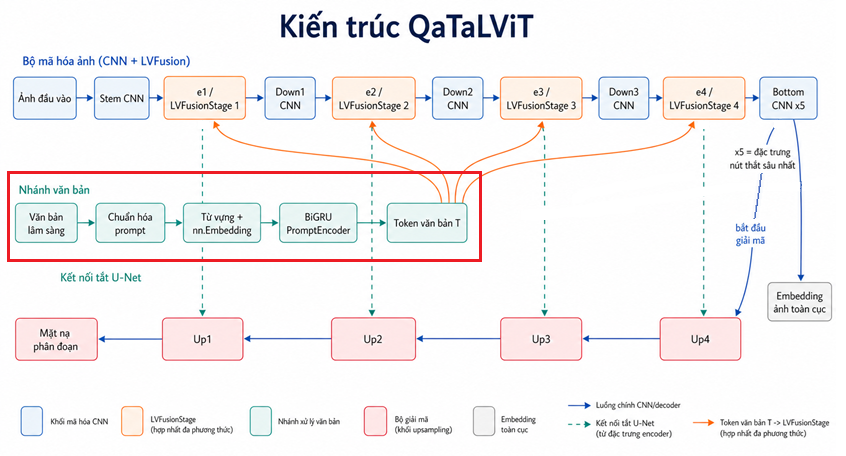
\includegraphics[width=0.96\textwidth,height=#1,keepaspectratio]{assets/final_diagram_LViT_vi_text.png}}%
}

\newcommand{\archfigCNN}[1][0.68\textheight]{%
  \makebox[\textwidth][c]{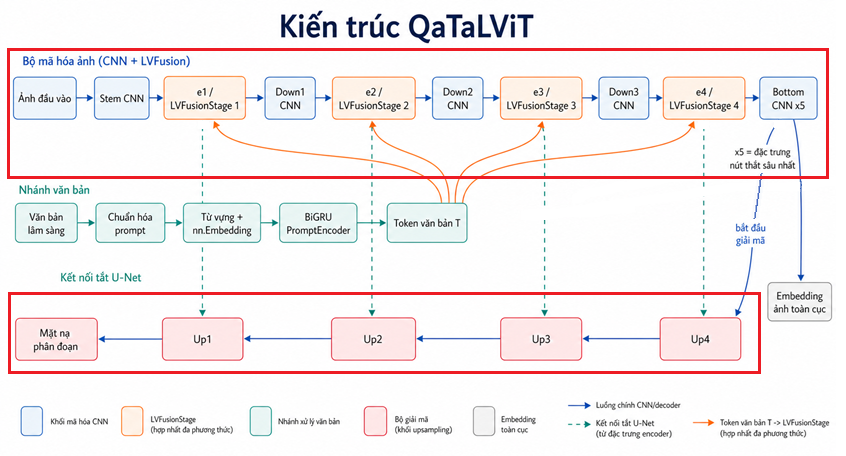
\includegraphics[width=0.96\textwidth,height=#1,keepaspectratio]{assets/final_diagram_LViT_vi_CNN.png}}%
}

\newcommand{\mechfigfusion}[1][0.68\textheight]{%
  \makebox[\textwidth][c]{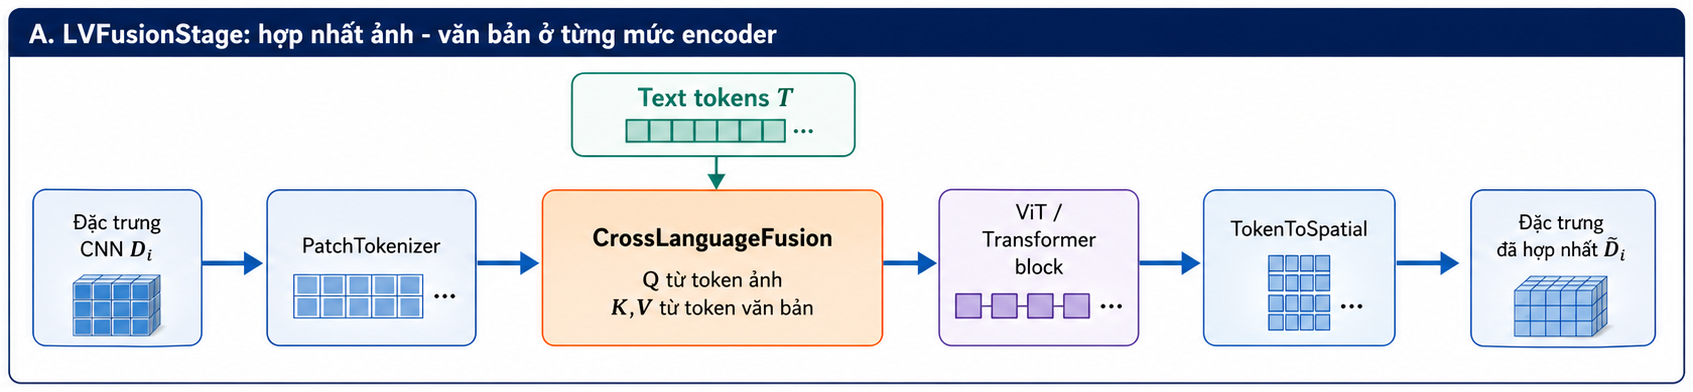
\includegraphics[width=0.96\textwidth,height=#1,keepaspectratio]{assets/LVFusion.png}}%
}

\newcommand{\mechfigema}[1][0.68\textheight]{%
  \makebox[\textwidth][c]{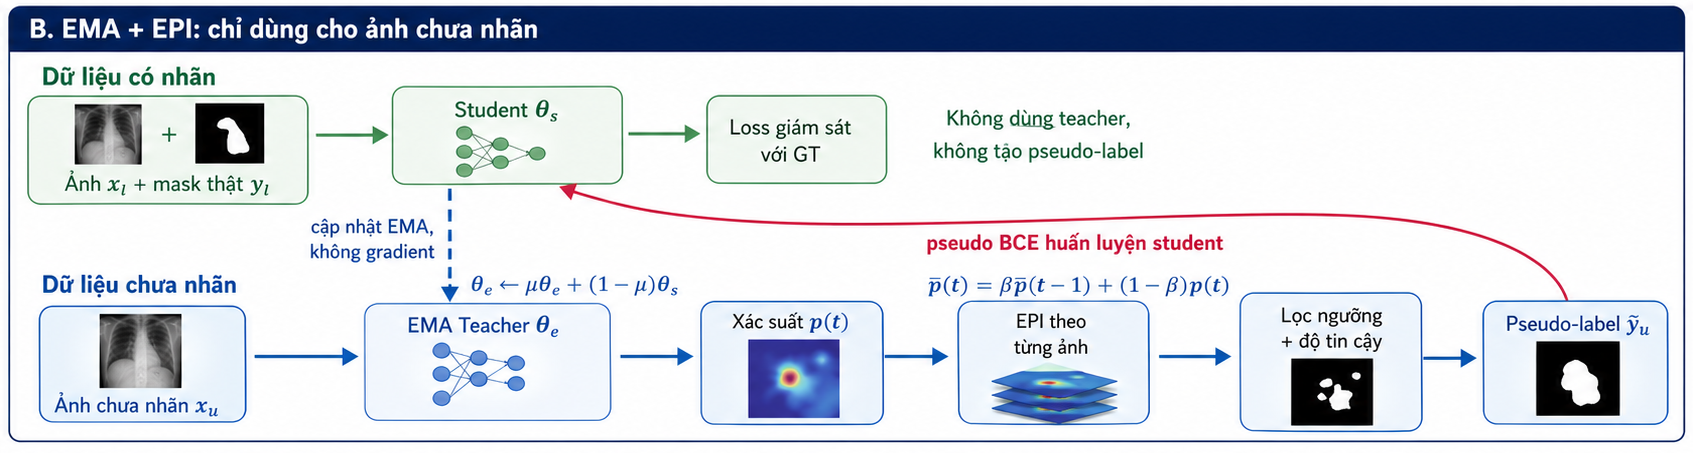
\includegraphics[width=0.96\textwidth,height=#1,keepaspectratio]{assets/EMA.png}}%
}

\newcommand{\shortcue}[1]{%
  \vspace{0.12cm}
  {\small\color{ink}#1}
}

\newcommand{\summaryframe}[2]{%
  \begin{frame}{#1}
    \vspace{0.25cm}
    \makebox[\textwidth][c]{%
      \begin{beamercolorbox}[wd=0.86\textwidth,rounded=true,sep=0.28cm]{block body}
        #2
      \end{beamercolorbox}%
    }
  \end{frame}
}

\title[QaTaLViT]{QaTaLViT}
\subtitle{Phân đoạn ảnh y khoa kết hợp văn bản với dữ liệu hạn chế}
\author[Bộ môn Thị giác Máy tính]{Lưu Huy Minh Quang -- 23127016\\Trương Quốc Cường -- 23127333}
\institute[HCMUS]{Trường Đại học Khoa học Tự nhiên -- ĐHQG TP.HCM}
\date{}

\begin{document}

\begin{frame}[plain]
  \centering
  \vspace{0.9cm}
  \makebox[\textwidth][c]{%
    \begin{beamercolorbox}[wd=0.86\textwidth,rounded=true,sep=0.45cm,center]{frametitle}
      {\LARGE\bfseries QaTaLViT\par}
      \vspace{0.22cm}
      {\large Phân đoạn ảnh y khoa kết hợp văn bản với dữ liệu hạn chế\par}
    \end{beamercolorbox}%

  }
  {\large  Lưu Huy Minh Quang -- 23127016\par}
  \vspace{0.2cm}
  {\large Trương Quốc Cường -- 23127333\par}
  \vspace{0.2cm}
  {\normalsize Trường Đại học Khoa học Tự nhiên -- ĐHQG TP.HCM\par}
\end{frame}




\summaryframe{Bài toán}{
\begin{itemize}
  \item Trong phân đoạn ảnh y khoa, nếu chỉ dùng ảnh làm nguồn tri thức duy nhất, mô hình thường gặp nhiều khó khăn.
  \item Biên tổn thương có thể mờ, vùng cần phân đoạn nhỏ và dễ lẫn với nền.
  \item Ảnh y khoa thay đổi theo thiết bị, quy trình chụp và nguồn dữ liệu ở từng nơi.
  \item Mask phân đoạn rất tốn công gán nhãn vì cần chuyên gia y tế thực hiện.
  \item Vì vậy, bài toán vừa khó về mặt thị giác, vừa khó do dữ liệu được gán nhãn đầy đủ thường khan hiếm.
\end{itemize}
}

\summaryframe{Ý tưởng chính}{
\begin{itemize}
  \item Ảnh y khoa thường đi kèm với mô tả hoặc chẩn đoán lâm sàng ngắn.
  \item Nguồn văn bản này dễ thu thập hơn mask phân đoạn và thường có cấu trúc tương đối rõ.
  \item Văn bản có thể chứa thông tin về bên phổi, vị trí tương đối, số vùng tổn thương và mức độ bất thường.
  \item Do đó, QaTaLViT tận dụng văn bản như tín hiệu ngữ cảnh bổ sung cho ảnh.
  \item Mục tiêu là dùng văn bản để định hướng đặc trưng ảnh, giúp mô hình tạo mask chính xác hơn.
\end{itemize}
}

\begin{frame}{Tổng quan hệ thống}
  \centering
  \vspace{0.15cm}
  \archfig[0.78\textheight]
\end{frame}

\summaryframe{Tóm tắt tổng quan}{
\begin{itemize}
  \item QaTaLViT giữ ảnh làm nguồn quyết định hình dạng mặt nạ, còn văn bản đóng vai trò gợi ý ngữ cảnh và vị trí tổn thương.
  \item Thực nghiệm dùng hai bộ dữ liệu: QaTa-COV19 với ảnh X-quang ngực và MosMedData+ với CT lát cắt.
  \item Hệ thống gồm bốn phần: nhánh văn bản, trục CNN kiểu U-Net, các tầng LVFusionStage/ViT, và nhánh EMA/EPI cho dữ liệu chưa nhãn.
  \item Kết quả chính luôn đọc cùng đối sánh: QaTa-COV19 50\% đạt 84.03 / 75.62, cao hơn LViT-T 82.73 / 73.99; MosMedData+ 50\% đạt 73.84 / 60.31, nhỉnh hơn LViT-T về Dice nhưng còn thấp hơn về mIoU.
  \item MosMedData+ được dùng như thí nghiệm mở rộng 50\% nhãn, vì đây là mức cân bằng giữa mặt nạ thật và dữ liệu chưa nhãn để kiểm tra pseudo-label.
\end{itemize}
}

\begin{frame}{Phần 1: Nhánh văn bản}
  \centering
  \vspace{0.15cm}
  \archfigtext[0.78\textheight]
\end{frame}

\summaryframe{Tóm tắt nhánh văn bản}{
\begin{itemize}
  \item Đầu vào văn bản là mô tả lâm sàng ngắn, thường chứa thông tin về bên phổi, số vùng tổn thương và vị trí tương đối.
  \item Prompt normalization đưa các cách viết khác nhau về dạng ổn định hơn, giúp mô hình không phải học quá nhiều biến thể ngôn ngữ không cần thiết.
  \item Prompt sau chuẩn hóa được ánh xạ qua từ vựng, \texttt{nn.Embedding} và BiGRU PromptEncoder để tạo token văn bản \(T\).
  \item Token \(T\) không trực tiếp sinh mask, mà được dùng làm tín hiệu điều hướng cho các tầng LVFusionStage.
\end{itemize}
}

\begin{frame}{Phần 2: Trục CNN kiểu U-Net}
  \centering
  \vspace{0.15cm}
  \archfigCNN[0.78\textheight]
\end{frame}

\summaryframe{Tóm tắt trục CNN}{
\begin{itemize}
  \item CNN encoder là xương sống chính để giữ chi tiết không gian, biên tổn thương và cấu trúc cục bộ của ảnh.
  \item Ảnh đi qua Stem, Down1, Down2, Down3 và Bottom để tạo các đặc trưng nhiều mức \(e_1..e_4\) và bottleneck \(x_5\).
  \item Decoder dùng \(Up4 \rightarrow Up1\) để tăng dần độ phân giải và khôi phục mặt nạ phân đoạn.
  \item Skip connection nối encoder với decoder, nhưng trong QaTaLViT các skip feature đã được tinh chỉnh bởi văn bản trước khi đưa vào decoder.
\end{itemize}
}

\begin{frame}{Phần 3: LVFusionStage và ViT}
  \centering
  \vspace{0.15cm}
  \mechfigfusion[0.78\textheight]
\end{frame}

\summaryframe{Tóm tắt LVFusionStage}{
\begin{itemize}
  \item LVFusionStage là nơi tương tác ảnh--văn bản diễn ra trực tiếp trên đặc trưng encoder ở nhiều mức.
  \item Feature CNN \(D_i\) được token hóa bằng PatchTokenizer; token ảnh đóng vai trò truy vấn, còn token văn bản \(T\) đóng vai trò khóa/giá trị trong CrossLanguageFusion.
  \item Sau chú ý chéo, token đã hợp nhất đi qua ViT/Transformer block để học quan hệ dài hơn, rồi TokenToSpatial chiếu ngược về feature map.
  \item Nhờ vậy, văn bản không thay thế CNN, mà điều chỉnh đặc trưng ảnh trước khi đặc trưng đó đi vào skip connection và decoder.
\end{itemize}
}

\begin{frame}{Phần 4: EMA và EPI}
  \centering
  \vspace{0.15cm}
  \mechfigema[0.78\textheight]
\end{frame}

\summaryframe{Tóm tắt EMA và EPI}{
\begin{itemize}
  \item Với dữ liệu có nhãn, student học trực tiếp từ ground truth; teacher không tạo nhãn cho phần này.
  \item Với dữ liệu chưa nhãn, EMA teacher là bản trung bình trượt của student, dùng để sinh xác suất dự đoán ổn định hơn.
  \item EPI lưu và làm mượt xác suất theo từng ảnh qua nhiều lần xuất hiện, giúp pseudo-label ít bị nhiễu bởi một mini-batch riêng lẻ.
  \item Sau khi lọc theo ngưỡng và độ tin cậy, pseudo-label quay lại huấn luyện student bằng pseudo BCE. Trong thực nghiệm MosMedData+, nhánh này cần rất thận trọng vì teacher yếu có thể làm kết quả xấu đi.
\end{itemize}
}

\begin{frame}{Kết quả trên QaTa-COV19}
  \centering
  \renewcommand{\arraystretch}{1.22}
  \begin{tabular}{lccc}
    \toprule
    Phương pháp & 25\% nhãn & 50\% nhãn & 100\% nhãn \\
    \midrule
    LViT huấn luyện lại & 78.42 / 68.43 & 80.32 / 70.60 & 82.76 / 73.78 \\
    LViT-T công bố & 80.95 / 71.31 & 82.73 / 73.99 & 83.66 / 75.11 \\
    QaTaLViT & \textbf{82.22 / 73.35} & \textbf{84.03 / 75.62} & \textbf{85.28 / 77.25} \\
    \bottomrule
  \end{tabular}

  \vspace{0.35cm}
  \small Mỗi ô là Dice / mIoU (\%). QaTaLViT vượt LViT-T công bố ở cả ba mức nhãn.
\end{frame}

\begin{frame}{Kết quả trên MosMedData+}
  \centering
  \renewcommand{\arraystretch}{1.22}
  \begin{tabular}{lccc}
    \toprule
    Phương pháp & Văn bản & Tỷ lệ nhãn & Dice / mIoU (\%) \\
    \midrule
    LViT-T chạy lại & Có & 50\% & 68.88 / 55.14 \\
    LViT-T công bố & Có & 50\% & 73.56 / 61.05 \\
    QaTaLViT tốt nhất & Có & 50\% & \textbf{73.84 / 60.31} \\
    \bottomrule
  \end{tabular}

  \vspace{0.25cm}
  \small QaTaLViT 50\% nhãn nhỉnh hơn LViT-T 50\% về Dice (73.84 so với 73.56), nhưng mIoU còn thấp hơn.

\end{frame}

\begin{frame}{Tài liệu tham khảo}
  \small
  \begin{thebibliography}{9}
    \bibitem{lvit}
    Li et al., \emph{LViT: Language meets Vision Transformer in Medical Image Segmentation}, IEEE TMI.

    \bibitem{qata}
    Degerli et al., QaTa-COV19 dataset and COVID-19 chest X-ray segmentation benchmark.

    \bibitem{mosmed}
    Morozov et al., MosMedData and MosMedData+ COVID-19 CT segmentation benchmark.

    \bibitem{nnunet}
    Isensee et al., \emph{nnU-Net: a self-configuring method for deep learning-based biomedical image segmentation}.
  \end{thebibliography}
\end{frame}

\end{document}
